\documentclass{beamer}

\usepackage{framed}
\usepackage{graphicx}

\usepackage{amsmath}

\begin{document}
	
%======================================== %	
\begin{frame}
	\begin{figure}
\centering
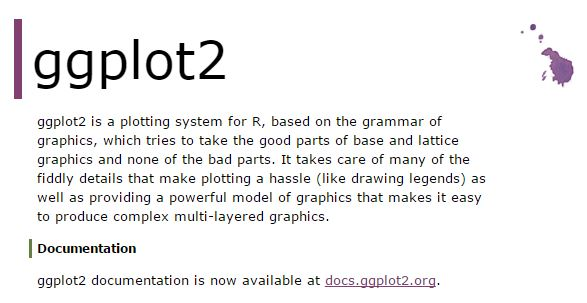
\includegraphics[width=1.1\linewidth]{ggplot2-website}
\end{figure}
website: www.had.co.nz

\end{frame}
%======================================== %
\begin{frame}
	\begin{figure}
\centering

\includegraphics[width=0.95\linewidth]{HW}

\end{figure}
Hadley Wickham (Chief Data Scientist, RStudio)
\end{frame}
%============================================= %

\begin{frame}
\begin{figure}
\centering
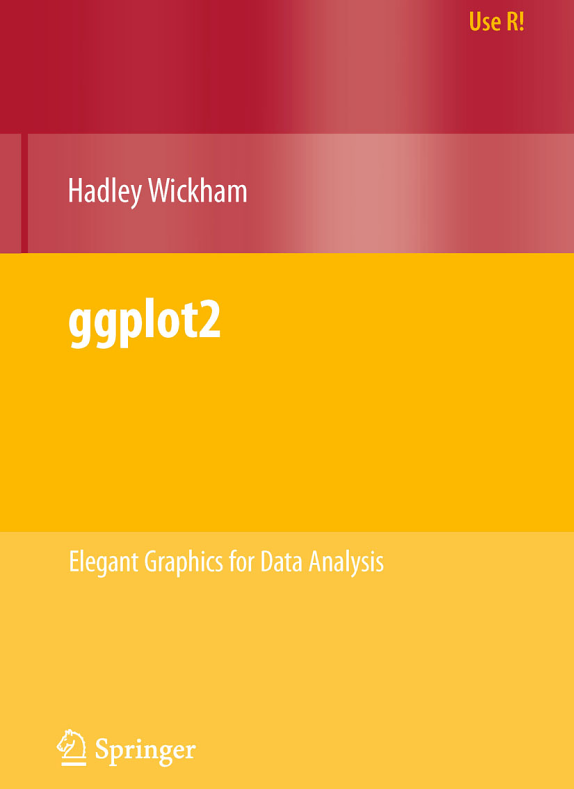
\includegraphics[width=0.55\linewidth]{ggplot2-bookcover}
\end{figure}
ggplot2: Elegant Graphics for Data Analysis
\end{frame}
%============================================= %

\begin{frame}
\begin{figure}
\centering
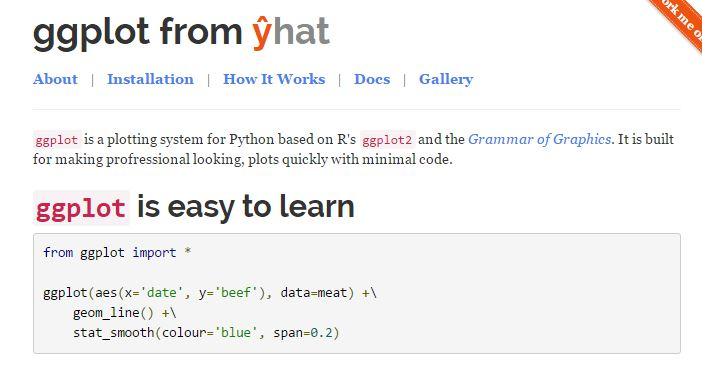
\includegraphics[width=1.1\linewidth]{ggplot-yhat}
\end{figure}
\Large
\noindent \textbf{Important :} \\ for Python, the name is simply ``\textbf{ggplot}".
\end{frame}
%============================================= %

\begin{frame}
	
\begin{figure}
\centering

\includegraphics[width=0.8\linewidth]{yhat}
\end{figure}
\Large
\textbf{Yhat} (\textit{pronounced y-hat}) is a data science technology company that provides tools and systems that allow enterprises to turn data insights into data-driven products.\\ \bigskip


\end{frame}
%======================================= %

\begin{frame}
	\Large
	\noindent\textbf{About ggplot}

	
\textbf{ggplot} is a graphics package for Python that aims to approximate R's ggplot2 package in both usage and aesthetics.\\
\bigskip
\textbf{Authors:} Greg Lamp and Austin Ogilvie
\end{frame}
%======================================= %

\begin{frame}
\Large
\noindent\textbf{What are Yhat saying?}

\begin{enumerate}
	\item ggplot is easy to learn [\textit{1}]
	\item ggplot is fun
	\item ggplot is powerful [\textit{2}]
\end{enumerate}

\begin{framed}
\textit{[1] Lots of learning resources, mainly intended for the R environment, that can applied to Python also.}\\
\bigskip
\textit{[2] Less code required to compute high-level publication quality plot}
\end{framed}
\end{frame}
%===================================== %
\begin{frame}[fragile]
\textbf{1. Installing ggplot}
\begin{framed}
\begin{verbatim}
pip install ggplot
\end{verbatim}
\end{framed}
\textbf{2. Getting Set Up on Jupyter Notebook}
\begin{figure}
\centering
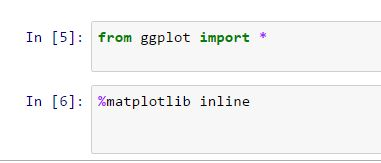
\includegraphics[width=0.7\linewidth]{jupyter1}
\end{figure}

\end{frame}
%===================================== %
\begin{frame}
	\Large
	\begin{figure}
\centering
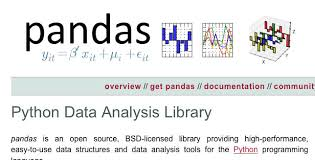
\includegraphics[width=0.7\linewidth]{pandas}
\end{figure}

	\textbf{Important:} ggplot accepts data in the form of a \texttt{pandas Dataframe}, so you need to configure all data accordingly first.
\end{frame}
%===================================== %
\begin{frame}[fragile]
	\Large
Watch out for this operator
\begin{framed}
\begin{verbatim}
.... +\ .....
\end{verbatim}
\end{framed}
	\begin{figure}
\centering
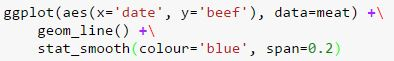
\includegraphics[width=1.05\linewidth]{plusoperator}
\end{figure}
\end{frame}
%===================================== %
\begin{frame}[fragile]
\Large
\begin{itemize}
\item The main command is \texttt{ggplot()}.
\item The name comes from "\textbf{grammar of graphics}", a book by Leland Wilkinson
\item A very ``high-level" approach to data visualization.
\end{itemize}
\begin{framed}
\begin{quote}
	A grammar of graphics is a tool that enables us to concisely describe the components
	of a graphic. Such a grammar allows us to move beyond named graphics (e.g., the “scatterplot”)
	and gain insight into the deep structure that underlies statistical graphics.
\end{quote}
\end{framed}
\end{frame}

\begin{frame}

\begin{figure}
\centering
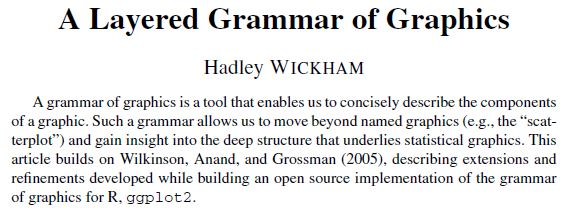
\includegraphics[width=1.1\linewidth]{HWpaper}
\end{figure}
\begin{framed}
Hadley Wickham.\\
\textbf{A layered grammar of graphics.}\\
\textit{Journal of Computational and Graphical Statistics, \\ vol. 19, no. 1, pp. 3–28, 2010.}
\end{framed}

\end{frame}
%===================================== %
\begin{frame}[fragile]
	\begin{figure}
\centering
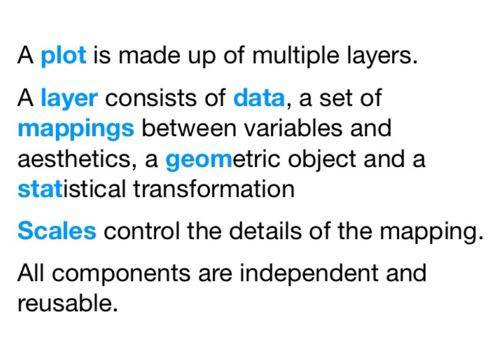
\includegraphics[width=1.1\linewidth]{ggplot2-info}
\end{figure}
(Source: Hadley Wickham)
\end{frame}



\end{document}
